% ****** Start of file apssamp.tex ******
%
%   This file is part of the APS files in the REVTeX 4.2 distribution.
%   Version 4.2a of REVTeX, December 2014
%
%   Copyright (c) 2014 The American Physical Society.
%
%   See the REVTeX 4 README file for restrictions and more information.
%
% TeX'ing this file requires that you have AMS-LaTeX 2.0 installed
% as well as the rest of the prerequisites for REVTeX 4.2
%
% See the REVTeX 4 README file
% It also requires running BibTeX. The commands are as follows:
%
%  1)  latex apssamp.tex
%  2)  bibtex apssamp
%  3)  latex apssamp.tex
%  4)  latex apssamp.tex
%
\documentclass[%
 % reprint,
%superscriptaddress,
%groupedaddress,
%unsortedaddress,
%runinaddress,
%frontmatterverbose, 
preprint,
%preprintnumbers,
%nofootinbib,
%nobibnotes,
%bibnotes,
 amsmath,amssymb,
 aps,
%pra,
%prb,
%rmp,
%prstab,
%prstper,
%floatfix,
]{revtex4-2}

\usepackage{graphicx}% Include figure files
\usepackage{dcolumn}% Align table columns on decimal point
\usepackage{bm}% bold math
\usepackage{hyperref}% add hypertext capabilities
%\usepackage[mathlines]{lineno}% Enable numbering of text and display math
%\linenumbers\relax % Commence numbering lines

% \usepackage[showframe,%Uncomment any one of the following lines to test 
% %scale=0.7, marginratio={1:1, 2:3}, ignoreall,% default settings
% %text={7in,10in},centering,
% %margin=1.5in,
% %total={6.5in,8.75in}, top=1.2in, left=0.9in, includefoot,
% %height=10in,a5paper,hmargin={3cm,0.8in},
% ]{geometry}

\begin{document}

\preprint{2023 Fall Global PhD Datathon}

\title{Are Good Headlines Simpler:\\A Study from the Upworthy Research Archive}

\author{Mingjiamei Zhang}
\affiliation{Department of Physics, The University of Chicago}

\date{\today}% It is always \today, today,
             %  but any date may be explicitly specified

%\keywords{Suggested keywords}%Use showkeys class option if keyword
                              %display desired
\maketitle

\section{Background and motivation}
\subsection{The Upworthy Research Archive}

Upworthy Research Archive is a dataset collected by Upworthy.com which covers the results of A/B tests from early 2013 into April 2015 \cite{matias2021upworthy}.
In each test, Upworthy randomly assigned different readers to see different packages which contains a headline and an image for the same story.
The content management system recorded the number of participants that were shown a given package (\textit{impressions}) and the number that clicked on the package (\textit{clicks}). 
After a period of time, an editor would review a dashboard that reported the results and either conduct an additional experiment (potentially with new packages) or choose which package to finalize for a given article. 
Editors sometimes finalized a package other than the best performing one. From that decision point, Upworthy would only display the final chosen package.

The \texttt{packages} dataset records the result of a series of tests.
Each test includes various number of packages with the same \texttt{test\_id} and for each package, the headline text \texttt{headline} and the \texttt{image\_id} are recorded as well as the associated number of \texttt{impressions} and \texttt{clicks}.
An example test with 4 packages is shown in Fig. \ref{fig:example_test}.

\subsection{Hypothesis: Simplicity affects the click rate}

Media creators always hope to attract more readers, but how to achieve it is usually unclear.
With the Upworthy Research Archive dataset, we hope to dig into the pattern of reader's response and help the media creator to craft more attractive headlines for their news articles.

What could be characteristics of attractive headlines?
Of course there are many possibilities.
\textbf{One intuition is that, the readers usually come from a diverse audience and the headlines that attract most shouldn't be too complicated to understand.
The simplicity (or, complexity) of the text will affect the response of the user.}

In the following report, we will dig into the dataset to find out what the relationship between the simplicity and the popularity.

\begin{figure}[!ht]
    \centering
    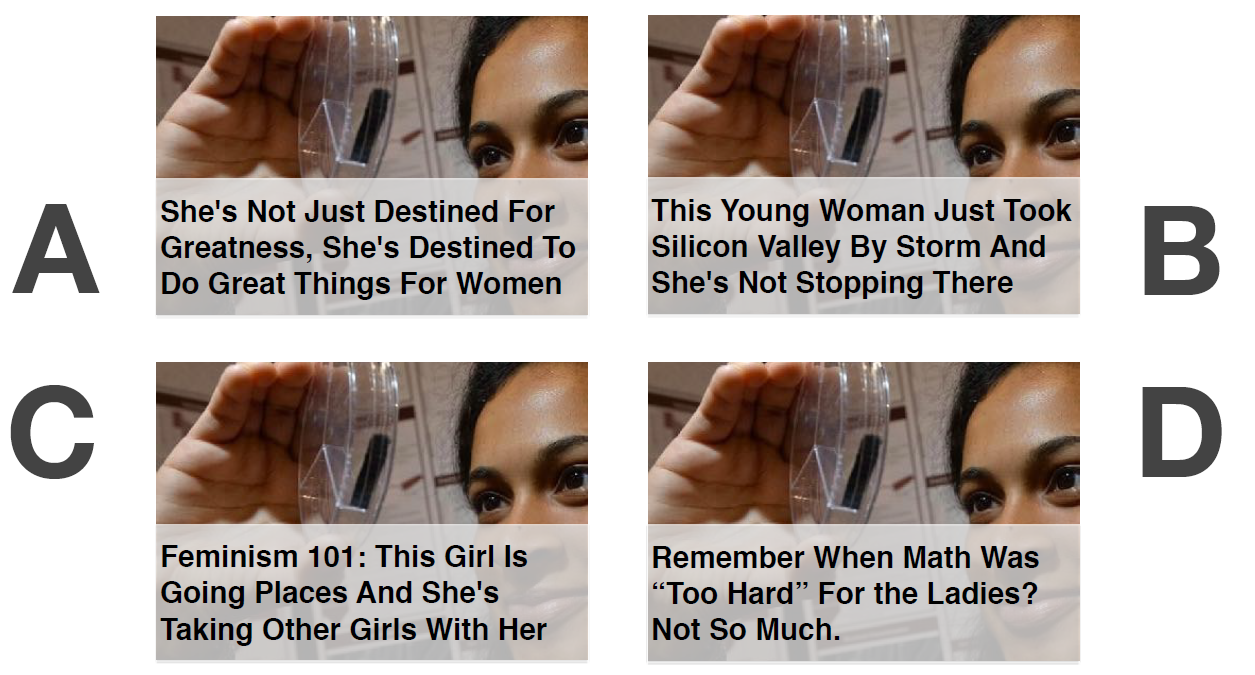
\includegraphics[width=0.8\linewidth]{fig/example_test.png}
    \caption{An example of a test of 4 packages (A, B, C, D). All packages have the same \texttt{test\_id} and are tested within the same week, but with potentially different images or headlines.}
    \label{fig:example_test}
\end{figure}

\section{Dataset statistics}

To get a feel of the dataset, we first perform exploratory data analysis on the \texttt{packages} dataset.
Since we are mostly interested in studying the effect of headlines, we dropped the entries that do not have valid headline information.
For all the remaining packages, as shown in Fig. \ref{fig:stat1_test_size}, most tests contain 2 to 8 packages with an average number of impression of about 3600 per package.

We denote a test as a set of packages, for example, a test \(t\) of \(n\) packages is \(t = \{p_1, p_2, ..., p_n\}\).
To see if the packages in the same test are being assigned to similar number of readers, we define the \textit{impression percentage difference} for a given test \(t\) as
\begin{equation}
   \texttt{max\_diff}_{t} = \frac{\mathrm{max}_{p\in t}(\texttt{impression}_p) - \mathrm{min}_{p\in t}(\texttt{impression}_p)}{\mathrm{mean}_{p\in t}(\texttt{impression}_p)}  
\end{equation}
which is the ratio of the maximum difference in impressions between two packages within the same test divided by the average impression for the test.
As shown in Fig. \ref{fig:stat2_package_imbalance}, for 99\% of the tests, the impression percentage difference is below 25\%, which means that most of the tests have relatively even impression distribution among packages.

We define \textit{click rate} for a given package \(p\) as
\begin{equation}
\label{eqn:click_rate}
    \texttt{click\_rate}_p = \frac{\texttt{clicks}_p}{\texttt{impressions}_p}    
\end{equation}
The distribution of click rates among packages is shown in Fig. \ref{fig:stat3_click_rate}, which indicates that most of the packages have a click rate of less than 7\%.
The average click rate among all packages in the dataset is
\begin{equation}
    \texttt{mean\_click\_rate} = \frac{\sum_{p\in\texttt{packages}} \texttt{clicks}_p}{\sum_{p\in\texttt{packages}} \texttt{impressions}_p}
\end{equation}
which is around 1.52\%.

\begin{figure}
    \centering
    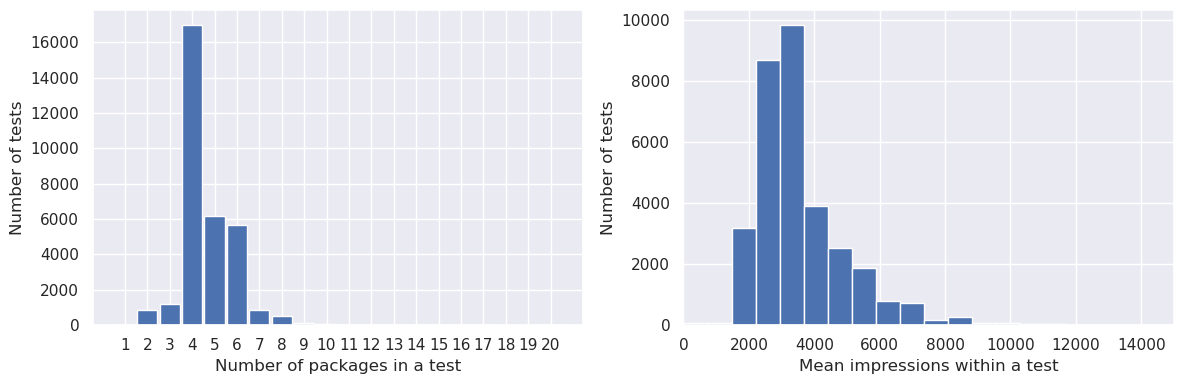
\includegraphics[width=\linewidth]{fig/stat1_test_size.png}
    \caption{Statistics of the tests. The left plot shows the number of tests with different number of containing packages. The right plot shows the number of tests with different average number of impression per package.}
    \label{fig:stat1_test_size}
\end{figure}

\begin{figure}
    \centering
    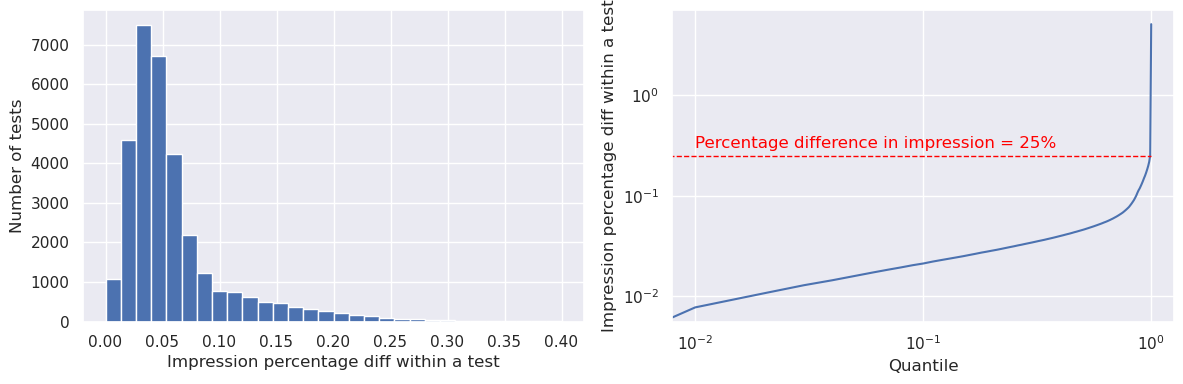
\includegraphics[width=\linewidth]{fig/stat2_package_impression_imbalance.png}
    \caption{Distribution of impression percentage difference. The left plot shows the distribution of impression percentage difference. The right plot is the quantile distribution. }
    \label{fig:stat2_package_imbalance}
\end{figure}

\begin{figure}
    \centering
    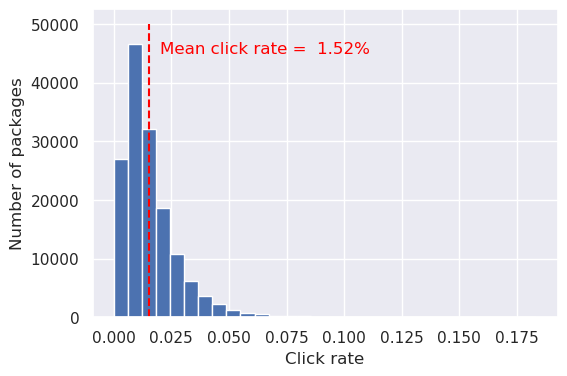
\includegraphics[width=0.5\linewidth]{fig/stat3_click_rate_hist.png}
    \caption{Distribution of click rate among all the packages with headlines.}
    \label{fig:stat3_click_rate}
\end{figure}

\section{Model of click rate}

\subsection{Simple model of reader's response}

To see if the difference in click rate between two packages in a test is significant, we developed a simple model of reader's response that takes into account of the number of samples (impressions) collected and the number of clicks received among the two packages.

The response of each reader is binary and stochastic, so we can model it as a Bernoulli random variable $X$ such that $X=1$ denotes that the user decides to click and $X=0$ is not to click.
To model the behavior of a group of readers exposed to the same package, we can make the following assumptions:
\begin{itemize}
    \item Each reader make choice of whether to click independently
    \item The probability of clicking is the same for all readers
\end{itemize}

The first assumption is reasonable because the readers are typically independent of each other. The second assumption is not very realistic since each reader should have his/her own preferences over topics/content, but it is a good approximation if the number of readers assigned for the package is large.

For a package with \(\texttt{impression}_k = N\), the number of received clicks \(Y = X_1 + X_2 + ... + X_N \) out of \(N\) readers is a binomial random variable with parameters \(N\) and \(p\), where $p$ is the probability of clicking on the package.
In practice, since the click rate is usually small (\(p\ll 1\)), we can use a Poisson distribution to approximate the binomial distribution, therefore the variance of \(Y\) is $Np$ which is the same as the expected value.

\subsection{Pairwise t-statistic of headline click rates}

From the observed clicks \(Y\), we can estimate the click rate of the package \(p\) as \(\hat{p} = Y/N\) and the variance of the estimate is \(\hat{p}/N\).
Given two packages 1 and 2 in the same test, the t-statistic of the difference in their click rates is then
\begin{equation}
    \texttt{t\_stat}_{1, 2} = \frac{\hat{p}_1 - \hat{p}_2}{\sqrt{\hat{p}_1/N_1 + \hat{p}_2/N_2}}
\end{equation}
where \(N_1\) and \(N_2\) are the impressions of the two packages respectively, and \(\hat{p}_1\) and \(\hat{p}_2\) are the estimated click rate of the two packages.
The t-statistic quantifies the statistical significance of the difference in click rates. 
With high absolute value of \texttt{t-stat}, we can say with strong confidence that the click rates are different.

Because the number of packages within a test could be more than two, we define the \textit{pairwise t-statistic} as the t-statistic of the difference in click rate between two packages within the test.
This way, a test of 4 packages with the same image but different headlines can generate \(\frac{4\times 3}{2} = 6\) pairs of headlines and corresponding pairwise t-statistic.

\subsection{Good headlines and bad headlines}

We define a \textit{good headline} is the headline in a pair of packages that results in higher click rate, and a \textit{bad headline} is the one with lower click rates.
To get a deeper understanding of what are the characteristics of good headlines and bad headlines, we compute the pairwise t-statistic of all pair of packages that are different \textit{only} by their headlines.
This way the difference in their click rate will only be due to the change in the headlines.

The total number of distinct pairs of headlines found is 140,621 across the \texttt{package} dataset with 63,209 unique headlines.
Within each pair, the headline with higher click rate is identified as a good headline while the other is a bad headline.
Since an actual test may contain more than two packages and a headline could be better than more than one headline in the same test, the same headline could appear many times as ``good headline" and is also possible to appear as ``bad headline" when compared to a stronger headline.
However, within each pair, the ``good headline" is always the one with higher click rate than the ``bad headline".
An example of 6 pairs of headlines with relatively high t-statistic is shown in Fig. \ref{fig:example_pairs}.

We can also look at the distribution of the pairwise t-statistic among all the 140,621 identified pairs of headlines.
As shown in Fig. \ref{fig:stat4_pairwise_t_stat}, the distribution is broader than a standard normal distribution with a standard deviation of \(\sigma = 1.967\), indicating that there are factors other than statistical fluctuation that contribute to the difference in click rates such that there are more pairs with high t-statistic than expected by assuming a normal distribution.

\begin{figure}
    \centering
    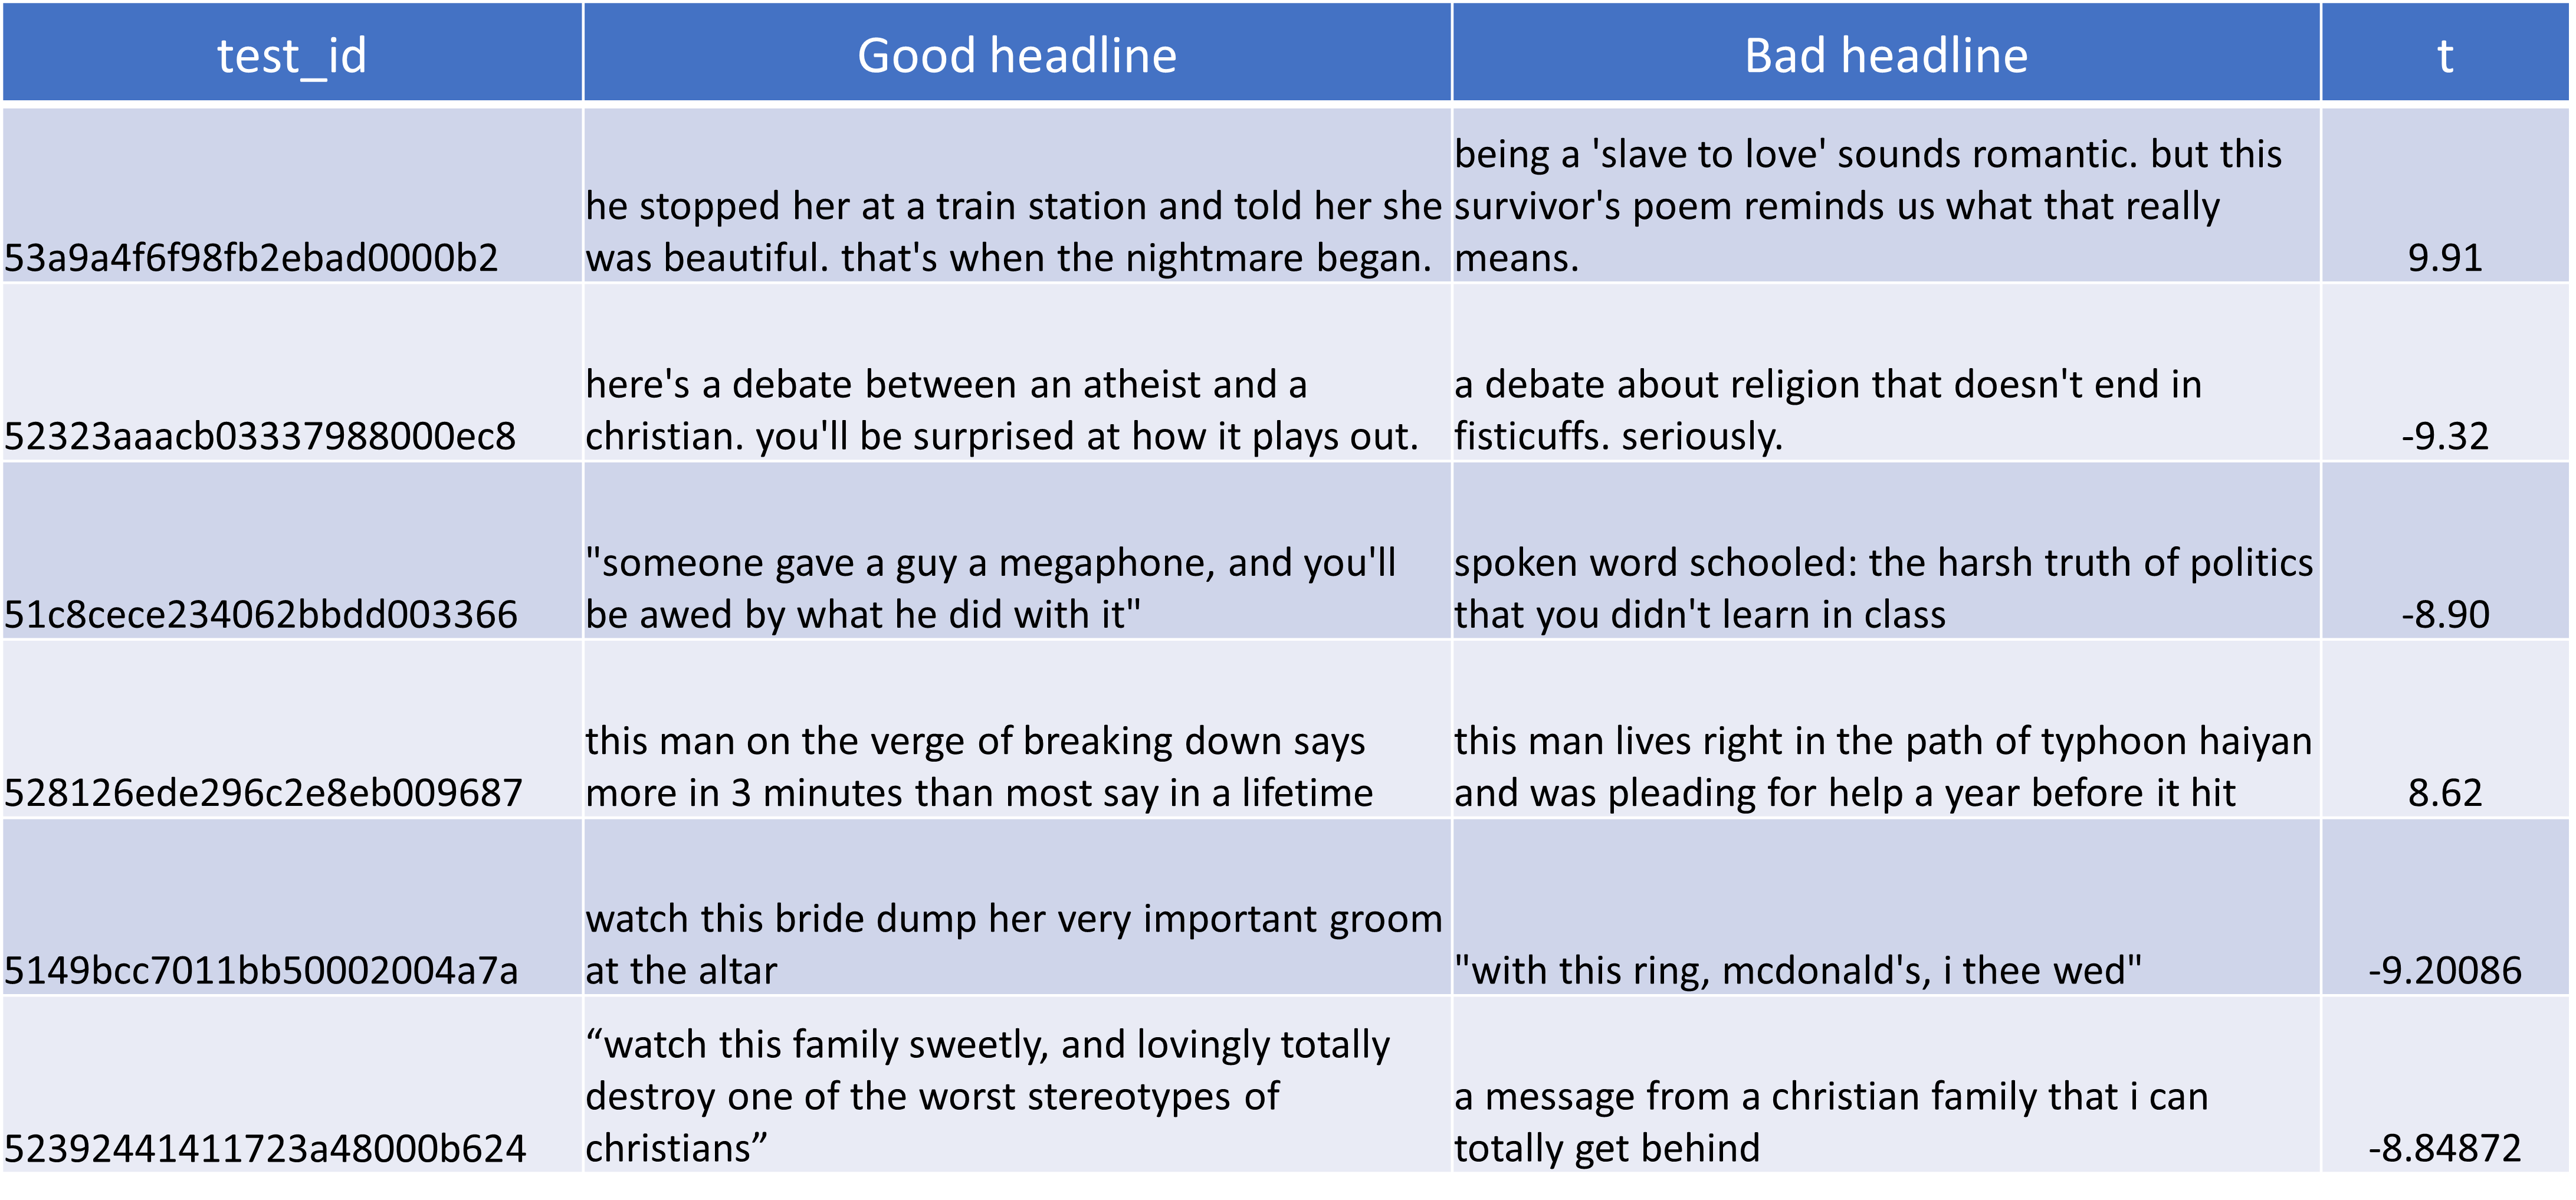
\includegraphics[width=\linewidth]{fig/example_pair_packages_headlines.png}
    \caption{Example of 6 pairs of headlines that result in different click rates. The t-statistic is evaluated with the order that the pair appear in the dataset, which could result in negative value if the package with good headline appears later.}
    \label{fig:example_pairs}
\end{figure}

\begin{figure}
    \centering
    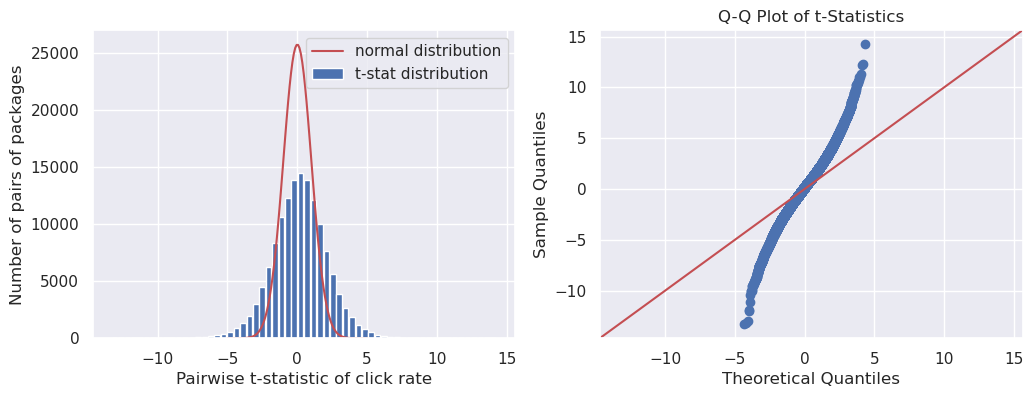
\includegraphics[width=\linewidth]{fig/stat4_pairwise_t-stat_hist.png}
    \caption{The distribution of pairwise t-statistic of the click rates across 140,621 pairs of packages that are different only by their headlines. Left plot shows the histogram of the distribution. Right plot shows the Q-Q plot of the distribution versus a standard normal distribution.}
    \label{fig:stat4_pairwise_t_stat}
\end{figure}

\section{Analysis}

% To study the relation of simplicity and click rate, we can ask the following two questions:
% \begin{enumerate}
%     \item Are the \textit{good} headlines typically \textit{simpler} than the bad headlines?
%     \item Are the \textit{simpler} headlines typically \textit{better}, i.e. receive higher click rates?
% \end{enumerate}

% For the first question, our approach is to identify and collect good headlines and bad headlines, and then analyze the richness and variety of the vocabulary.
% For the second question, we will assign a ``simplicity" score to each headline and study its effect on the click rate.

% -------------------------------------------------
Our question is: Are the \textit{good} headlines typically \textit{simpler} than the bad headlines?
To answer this question, our approach is to identify and collect good headlines and bad headlines, and then analyze the richness and variety of the vocabulary.
% -------------------------------------------------

% \subsection{Are good headlines simpler?}
\subsubsection{Collect good headlines and bad headlines with a set threshold}

With the pairwise t-statistic, we can collect a list of good headlines and a list of bad headlines and analyze the richness and variety of the vocabulary used in the two lists.

To do that, we define a threshold parameter \(\texttt{threshold} \geq 0\), such that only when the absolute value of the pairwise t-statistic is greater than the set threshold, we consider the good headline \textit{better} than the bad headline and put those two to the corresponding list.
The choice of threshold is a trade-off between the data size and the cleanness.
A higher threshold will result in a smaller data size for analysis because most of the headline pairs are filtered out, but can ensure that the good headlines are better than bad headlines with higher confidence level.
A lower threshold will preserve more headlines in the collected lists, but since it basically puts a headline to good headline list even if the higher click rate it receives is not statistically significant, it could potentially mix good and bad in the analysis.
As shown in Fig. \ref{fig:ttr1_threshold}, the number of headlines pairs decreases as the threshold increases.
When threshold is set to 5, the filtered pairs contain only about 2\% of the 140,621 pairs found in the original dataset.

If we consider each pair of headlines individually when constructing the lists, the same headline may appear multiple times in one list or even appear in both two lists, depending on the threshold value and its pairwise t-statistic with other headlines in the same test.
Although such repetition could be meaningful, we also consider constructing a \textit{unique} set of good headlines and bad headlines from the threshold-filtered list for analysis.

\begin{figure}
    \centering
    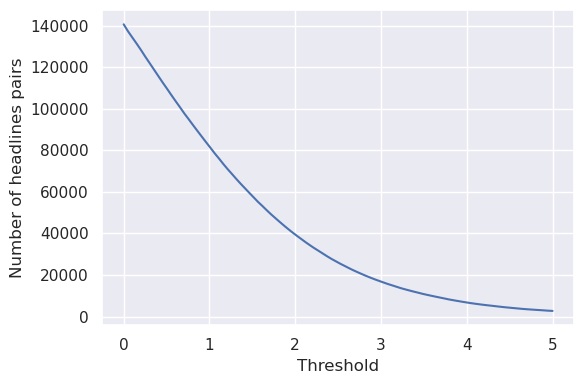
\includegraphics[width=0.5\linewidth]{fig/ttr1_threshold.png}
    \caption{The number of remaining headline pairs after applying a threshold filter on the absolute value of pairwise t-statistic.}
    \label{fig:ttr1_threshold}
\end{figure}

\subsubsection{Lexical diversity: Text-Token Ratio}

To quantitatively study the difference in the language used by the good and bad headlines, we can look into the \textit{Text-Token Ratio} (TTR) \cite{jurafskyspeech}.
TTR is a linguistic metric used to quantify the lexical diversity of a text or corpus which is calculated as the ratio of the total number of unique words (\textit{types}) to the total number of words (\textit{tokens}) in the given text, as defined below
\begin{equation}
    \texttt{TTR} = \frac{\mathrm{Number\ of\ types}}{\mathrm{Number\ of\ tokens}}
\end{equation}
TTR usually goes down as the number of tokens increases, which is because as more types are already included in the vocabulary, there is smaller chance to see a new type when including more tokens.
The corpus with less diversified vocabulary will typically have a lower TTR with the same token length, which means the number of unique words for a given number of words is lower.
A highly technical corpus is expected to have high TTR because lots of its words have low frequency.
As a reference, for English, it is usually sufficient to cover \(>90\%\) of the content with 2000 to 3000 types \cite{nagy1984many}.

We analyzed the TTR of the 4 headlines lists: \texttt{good}, \texttt{bad}, \texttt{good\_unique} and \texttt{bad\_unique}.
The lists are constructed with varying threshold parameter to filter the pairs and the unique headlines sets are constructed by removing repeated entries.
The lower-cased headlines are also pre-processed to remove punctuation and non-alphabetical words.
Fig. \ref{fig:ttr2_TTR} shows the TTR vs. number of tokens curves of the 4 groups and all of them show decreasing trend as token number increases. 
After the number of tokens reaches around 10k, the TTR starts to diverge between the 4 groups.
Since the TTR at low token number can fluctuate a lot, we look at the TTR at 20k tokens and find that the good (unique) headlines has a lower TTR than bad (unique) headlines with all threshold settings.
When the threshold is higher, the difference in TTR becomes larger and the TTR start to diverge at smaller token number, potentially due to the more distinct ``good" and ``bad" headlines included in the analysis.

To make sure the difference we see is statistically significant, we repeat the TTR measurement at 20k token number for 10 times by drawing random 20k tokens from the 4 groups. As shown in Fig. \ref{fig:ttr3_error_plot}, the TTR in the good headlines is consistently lower than in the bad headlines with or without the repeated headlines removed.
We can compute the t-statistic of the difference in TTR as
\begin{equation}
    t_{\mathrm{TTR}} = \frac{\mathrm{mean}(\mathrm{TTR}_{bad}) - \mathrm{mean}(\mathrm{TTR}_{good})}{\sqrt{\mathrm{var}(\mathrm{TTR}_{good}) + \mathrm{var}(\mathrm{TTR}_{bad})}}
\end{equation}
where the mean and var are taken among the 10 random draws.
Between \texttt{good} and \texttt{bad} headline lists, for all the threshold settings, the t-statistic is greater than 4.2 which indicates statistical significance of the difference in TTR.
For the \texttt{good\_unique} and \texttt{bad\_unique} lists, the t-statistic is 1.05 when threshold is set at 0, which is not significant (\(p > 0.05\)).
However, with higher threshold (\(\geq 2\)), the t-statitic is larger than 2.3 which indicates the significance in the difference in TTR.

When threshold is set to 2, for every 20k tokens (words), the \texttt{bad} headlines include on average 3709 types, while the \texttt{good} headlines include 3347 types, which is about 10\% lower.
If repeated headlines removed from the list, the \texttt{bad\_unique} headlines include 3745 types, while the \texttt{good\_unique} headlines include 3510 types, which is still about 6\% lower.
Since the difference is statistically significant, we can conclude that the better headlines are using less diversified words.

\begin{figure}
    \centering
    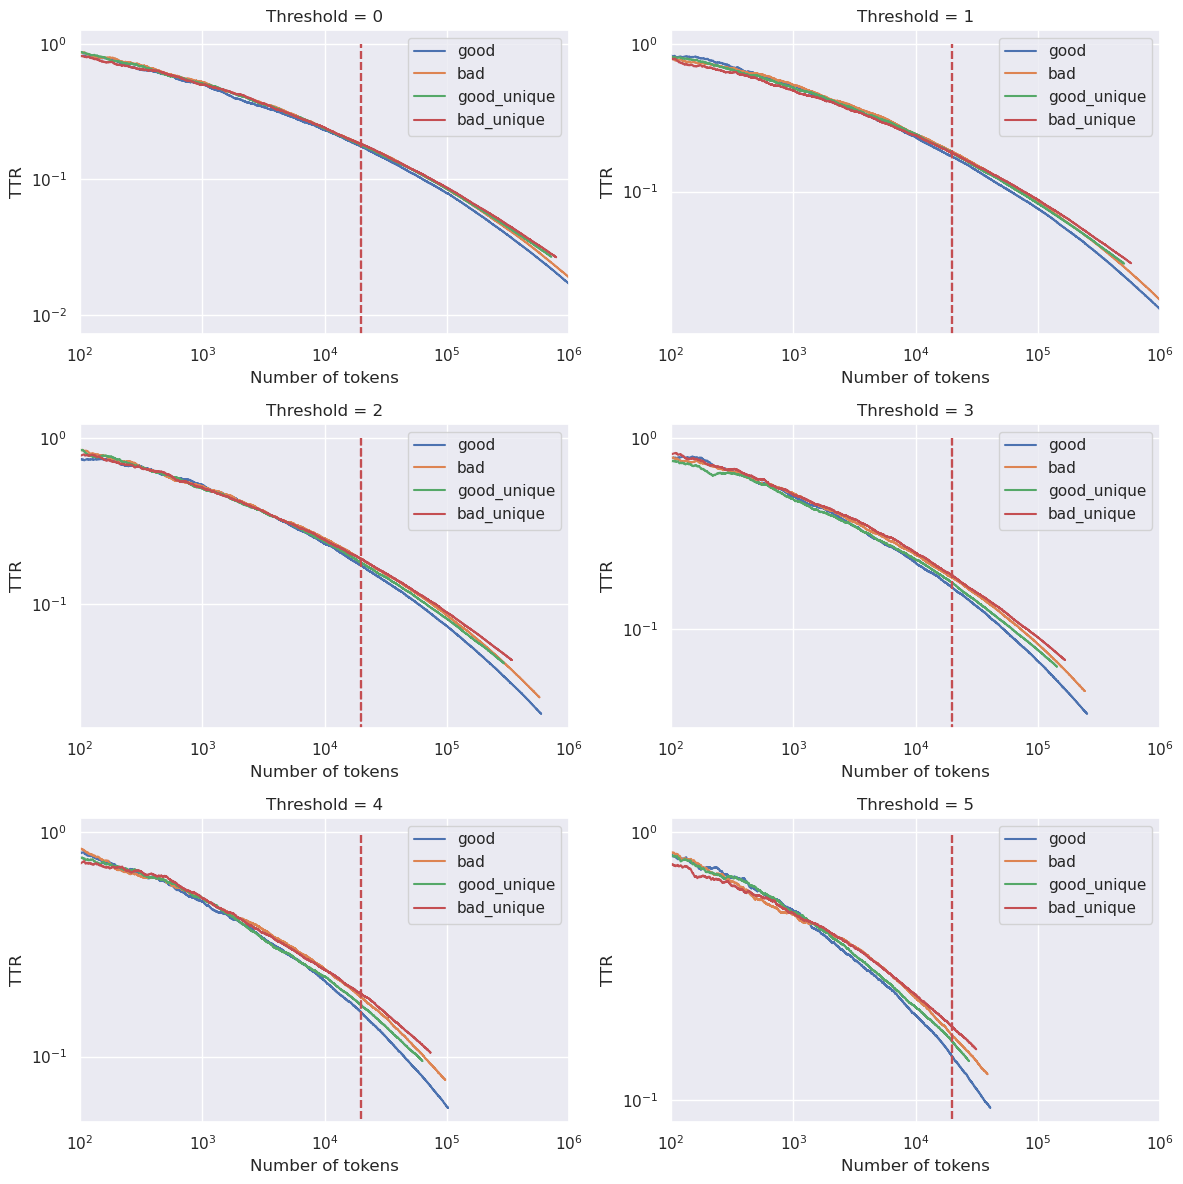
\includegraphics[width=\linewidth]{fig/ttr2_TTR_with_threshold.png}
    \caption{The Type-Token Ratio as a function of number of tokens between different groups of texts. Different plots are with different threshold setting for constructing good/bad headline lists. The ``good\_unique" and ``bad\_unique" are the unique headlines from the good/bad headline lists. As the threshold increases, the number of tokens included in the headline lists decreases, so the maximum number of tokens is different between the plots. As a reference, the red dash line marked the position of 20,000 tokens.}
    \label{fig:ttr2_TTR}
\end{figure}

\begin{figure}
    \centering
    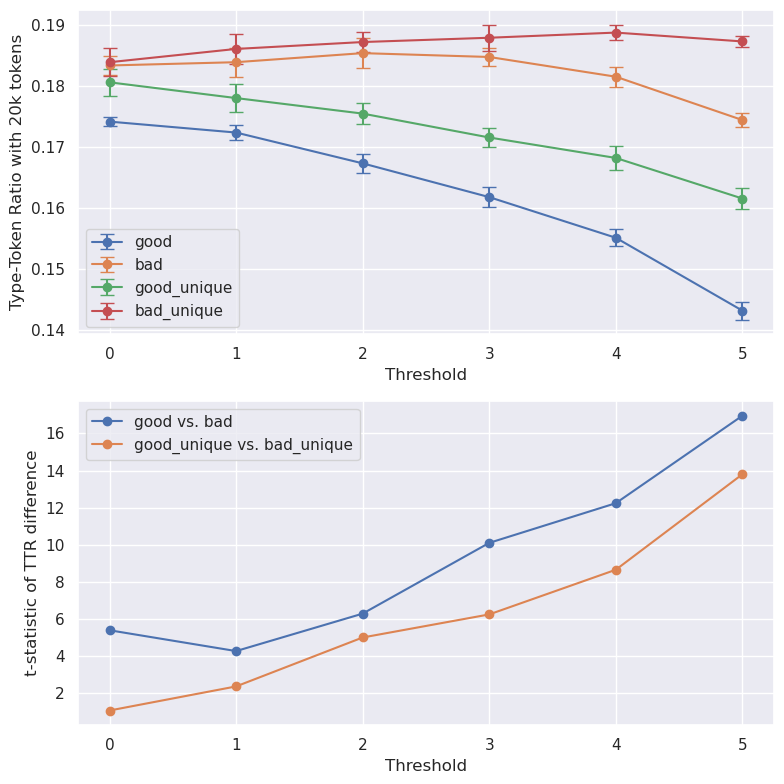
\includegraphics[width=0.8\linewidth]{fig/ttr3_error_plot.png}
    \caption{The Type-Token Ratio with 20k tokens for different groups of headlines. The upper plot shows the measured TTR with different threshold settings, where the value is obtained by averaging 10 repetitions, and the error bar denotes one standard deviation among the 10 measurements. The lower plot shows the t-statistic of the difference in TTR between \texttt{good} vs. \texttt{bad} and \texttt{good\_unique} vs. \texttt{bad\_unique}.}
    \label{fig:ttr3_error_plot}
\end{figure}

% \subsection{Are simpler headlines better?}
\subsubsection{The effect of less frequent words in a headline}

We can also study the effect of less frequent words in a headline.
From the previous analysis, we see that the good headlines typically use a smaller vocabulary, then a natural expectation is that, if a headline contains very infrequent words, it is less likely to be a good headline.

To study the effect of less frequent words in a headline on the click rate, we first build a word frequency table from all the unique headlines in the dataset.
The word frequency of a certain word \(w\) is then defined as
\begin{equation}
    \texttt{freq}(w) = \frac{\mathrm{Number\ of\ times\ the\ word\ } w\mathrm{\ appear\ in\ all\ headlines}}{\mathrm{Total\ number\ of\ words\ in\ all\ headlines}}
\end{equation}
An example of a few most frequent words and least frequent words is shown as a wordcloud in Fig. \ref{fig:wordcloud_most} and Fig. \ref{fig:wordcloud_least}.
The most frequent words are dominated by the pronouns and prepositions, and the least frequent words are usually more specific in meanings and sometimes include words that are misspelled or very confusing to people.
The most frequent 3000 words among the headlines constitute over 90\% of the total word counts.

\begin{figure}
    \centering
    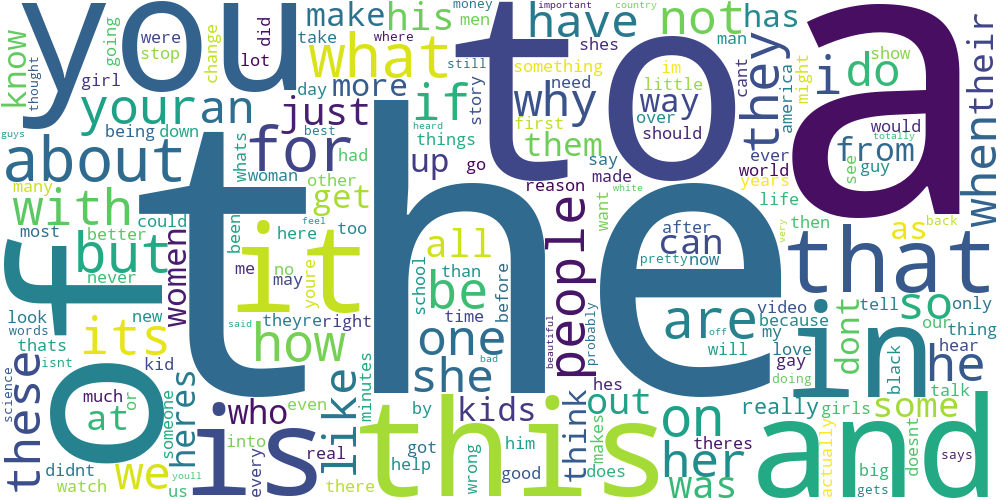
\includegraphics[width=0.8\linewidth]{fig/wordcloud1_most_frequent.png}
    \caption{The most frequent words in the headlines. The font size is ranked by the word frequency.}
    \label{fig:wordcloud_most}
\end{figure}

\begin{figure}
    \centering
    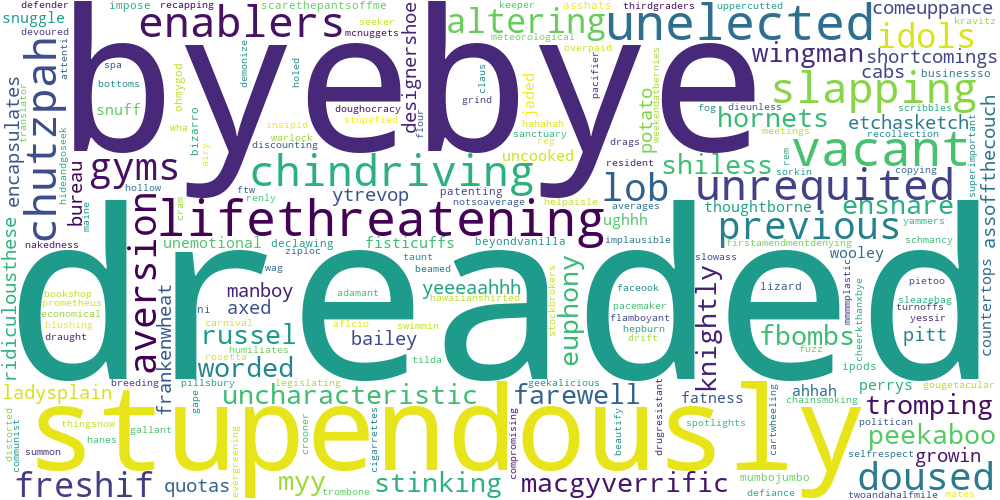
\includegraphics[width=0.8\linewidth]{fig/wordcloud2_least_frequent.png}
    \caption{The least frequent words in the headlines. the font size is ranked by the inverse of word frequency.}
    \label{fig:wordcloud_least}
\end{figure}

We define a headline ``infrequent" score as the minimum value of log of the frequency of the words occurred in the text
\begin{equation}
    \texttt{score}(headline) = \mathrm{min}_{w\in headline}\left\{\mathrm{log}(\texttt{freq}(w))\right\}
\end{equation}
This score is related to the frequency of least frequent word in a headline, so if the headline includes a very infrequent word, its score will be lower.
For every pair of headlines, we can define a score difference as the difference in the score between the two headlines
\begin{equation}
    \texttt{score\_diff}(A, B) = \texttt{score}(A) - \texttt{score}(B)
\end{equation}
The distribution of headline scores among the good and bad headline is shown in Fig. \ref{fig:score_diff}, where the threshold is set to 0.
The histogram shows a slight trend that the bad headlines are more likely to have lower score.

To study if the difference in the ``infrequent" score explains the difference in click rates, we plot the scatter plots of the score difference and pairwise t-statistic in Fig. \ref{fig:score_diff} and perform a least square fit \(Y \sim X\) where \(X\) is the score difference, and \(Y\) is the pairwise t-statistic in click rates.
The fit has an slope of \(0.0954\) and an \(R^2 = 0.01\), which means that about 1\% of the variation in the t-statistic can be explained by the score difference.
Although the \(R^2\) is small, the positive slope is significant above 0 with a t-statistic of 38.6, indicating a positive correlation with high confidence.

\begin{figure}
    \centering
    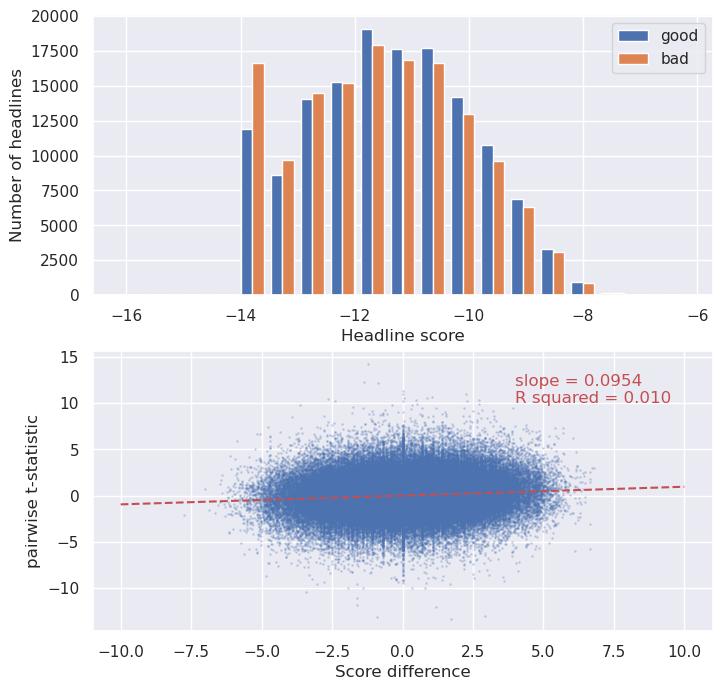
\includegraphics[width=0.8\linewidth]{fig/score_diff.png}
    \caption{The upper plots show the distribution of headline scores among \texttt{good} headlines and \texttt{bad} headlines if setting the threshold to be 0. The lower plot shows the scatter plot of score difference between a pair of headlines and their pairwise t-statistic of the click rates. The red dash line is a fit by linear regression with ordinary least square.}
    \label{fig:score_diff}
\end{figure}

\section{Conclusion}

From the Upworthy Research Archive dataset, we collected 140,621 pairs of packages that are different only by their headlines.
By analyzing the good headlines (with higher click rates) and bad headlines, we find that the good headlines are composed with a less diversified vocabulary, which is reflected on their relatively lower Type-Token Ratio.
We also find that the variation in the click rate difference can be partially explained by the ``infrequent" score of a headline, which further strengthens the claim that the appearance of a less frequent word negatively affects the performance of a headline.
Such finding indicates that \textit{simplicity} is a common feature of good headlines.

In the future, more study could be carried on to find more features of good headlines.

\bibliography{ref}% Produces the bibliography via BibTeX.

\end{document}
